\documentclass{article}

\begin{document}

\section{Introduction}

\section{Previous Work}

\section{System Description}

Existing electronic navigation aids have typically struggled to gain market traction and replace the traditional walking cane as the standard assistive tool for people with visual impairments.
Current technological limitations include prohibitive costs, bulky hardware requirements and non-user-friendly interfaces~\cite{golledge2004stated,yusif2016older,arditi2013user}.
To address these issues, we implemented a handheld mobile system that is based on a concept proposed in~\cite{lock2017portable,lock2019active} and tested in~\cite{lock2019bone} that uses a Google Tango device that is able to localise itself in real-time.
This system has the benefit of minimal hardware requirements and a compact, familiar form-factor, which will help to overcome the hurdle of user-acceptance and usability.

A set of bone-conduction headphones is used as the audio transmission medium.
These headphones sit on a user's cheekbones and conduct the audio signals through the skull into the inner ear, instead of through the outer part like typical over-ear headphones. 
This has the benefit of allowing the user access to ambient sounds and noise, so a person with limited vision can still relies on sound to detect, for example, oncoming vehicles and people~\cite{lichtenstein2012headphone}.
Alternative solutions, such as open-back headphones, were also considered.
These allow ambient noise through, but they still filter the incoming sound.
The AfterShockz headphones (\cref{fig:tango-headphone}) were ultimately selected since they do not interfere on other sounds and are also more discreet than the larger over-ear headphones. 

\subsection{Audio Interface}

Humans localise a sound source in 3 dimensions by considering cues recorded in one ear (monaural cues) and comparing cues received at both ears (binaural cues)~\cite{blauert1997spatial,blauert1969sound}.
The binaural cues include inter-aural time and level differences (ITD and ILD respectively) that help to determine a source's location on the horizontal plane.
Monaural cues are taken from the interaction of the sound with the human anatomy, e.g.\ head, shoulders, outer ear, before it enters the ear canal.
When the modified audio signal enters the inner ear canal, the human brain is able to analyse the frequency response and accurately determine the position of the sound source on the median plane. 
The distance to the source is simply derived as the intensity, or volume, of the source, i.e.\ a louder sound would appear closer to the user than a softer one. 

When an audio signal is transmitted via a set of speakers or headphones, it can be transformed with an HRTF to mimic the characteristics of a natural sound source before it is transmitted, tricking the brain into believing a sound is located at some arbitrary position.
An HRTF is a mathematical function that simulates the response signal of a human head and is derived by capturing key characteristics that affect the monaural and binaural responses, such as the user's hearing levels and head size.
Since hearing responses are unique amongst different users, the best results would be observed if each user had their own customised HRTF.\
However, given the complicated process involved to capture the required user characteristics, making unique HRTFs is often an untenable solution and using average values (e.g.\ head measurements, height, etc.) have shown to produce acceptable results~\cite{gardner1995hrtf}.

The guidance information is presented to the user in terms of pan and elevation angles, indicating the angular adjustments required to point the device camera at the target location, as shown in \cref{fig:cam-coords}.
Spatialised audio signals are well-suited to the task, displaying similar levels of performance to vocal feedback, but with less cognitive load and higher resolution~\cite{klatzky2006cognitive}.
However, given the previously discussed limitations of bone-conduction and spatialised audio, we propose a simple linear adjustment to the signal's pitch as a function of the elevation angle. 
The pan angle, instead, can be conveyed by transforming the audio signal with an HRTF, and indeed it has been found that this dimension is unaffected by using bone-conduction headphones\cite{schonstein2008comparison,macdonald2006spatial,stanley2006lateralization}. 

\begin{figure}[t]
  \centering
  \subfloat[]{\label{fig:cam-coords}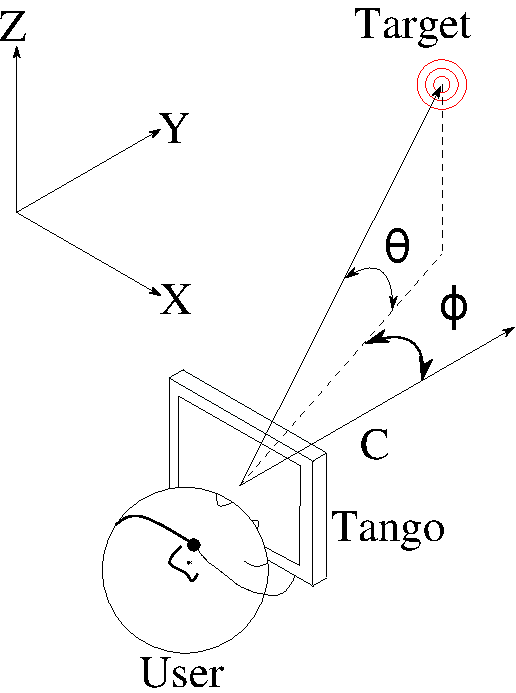
\includegraphics[width=0.3\columnwidth]{figures/camera_coordinate.pdf}}
~
  \subfloat[]{\label{fig:pitch-gain}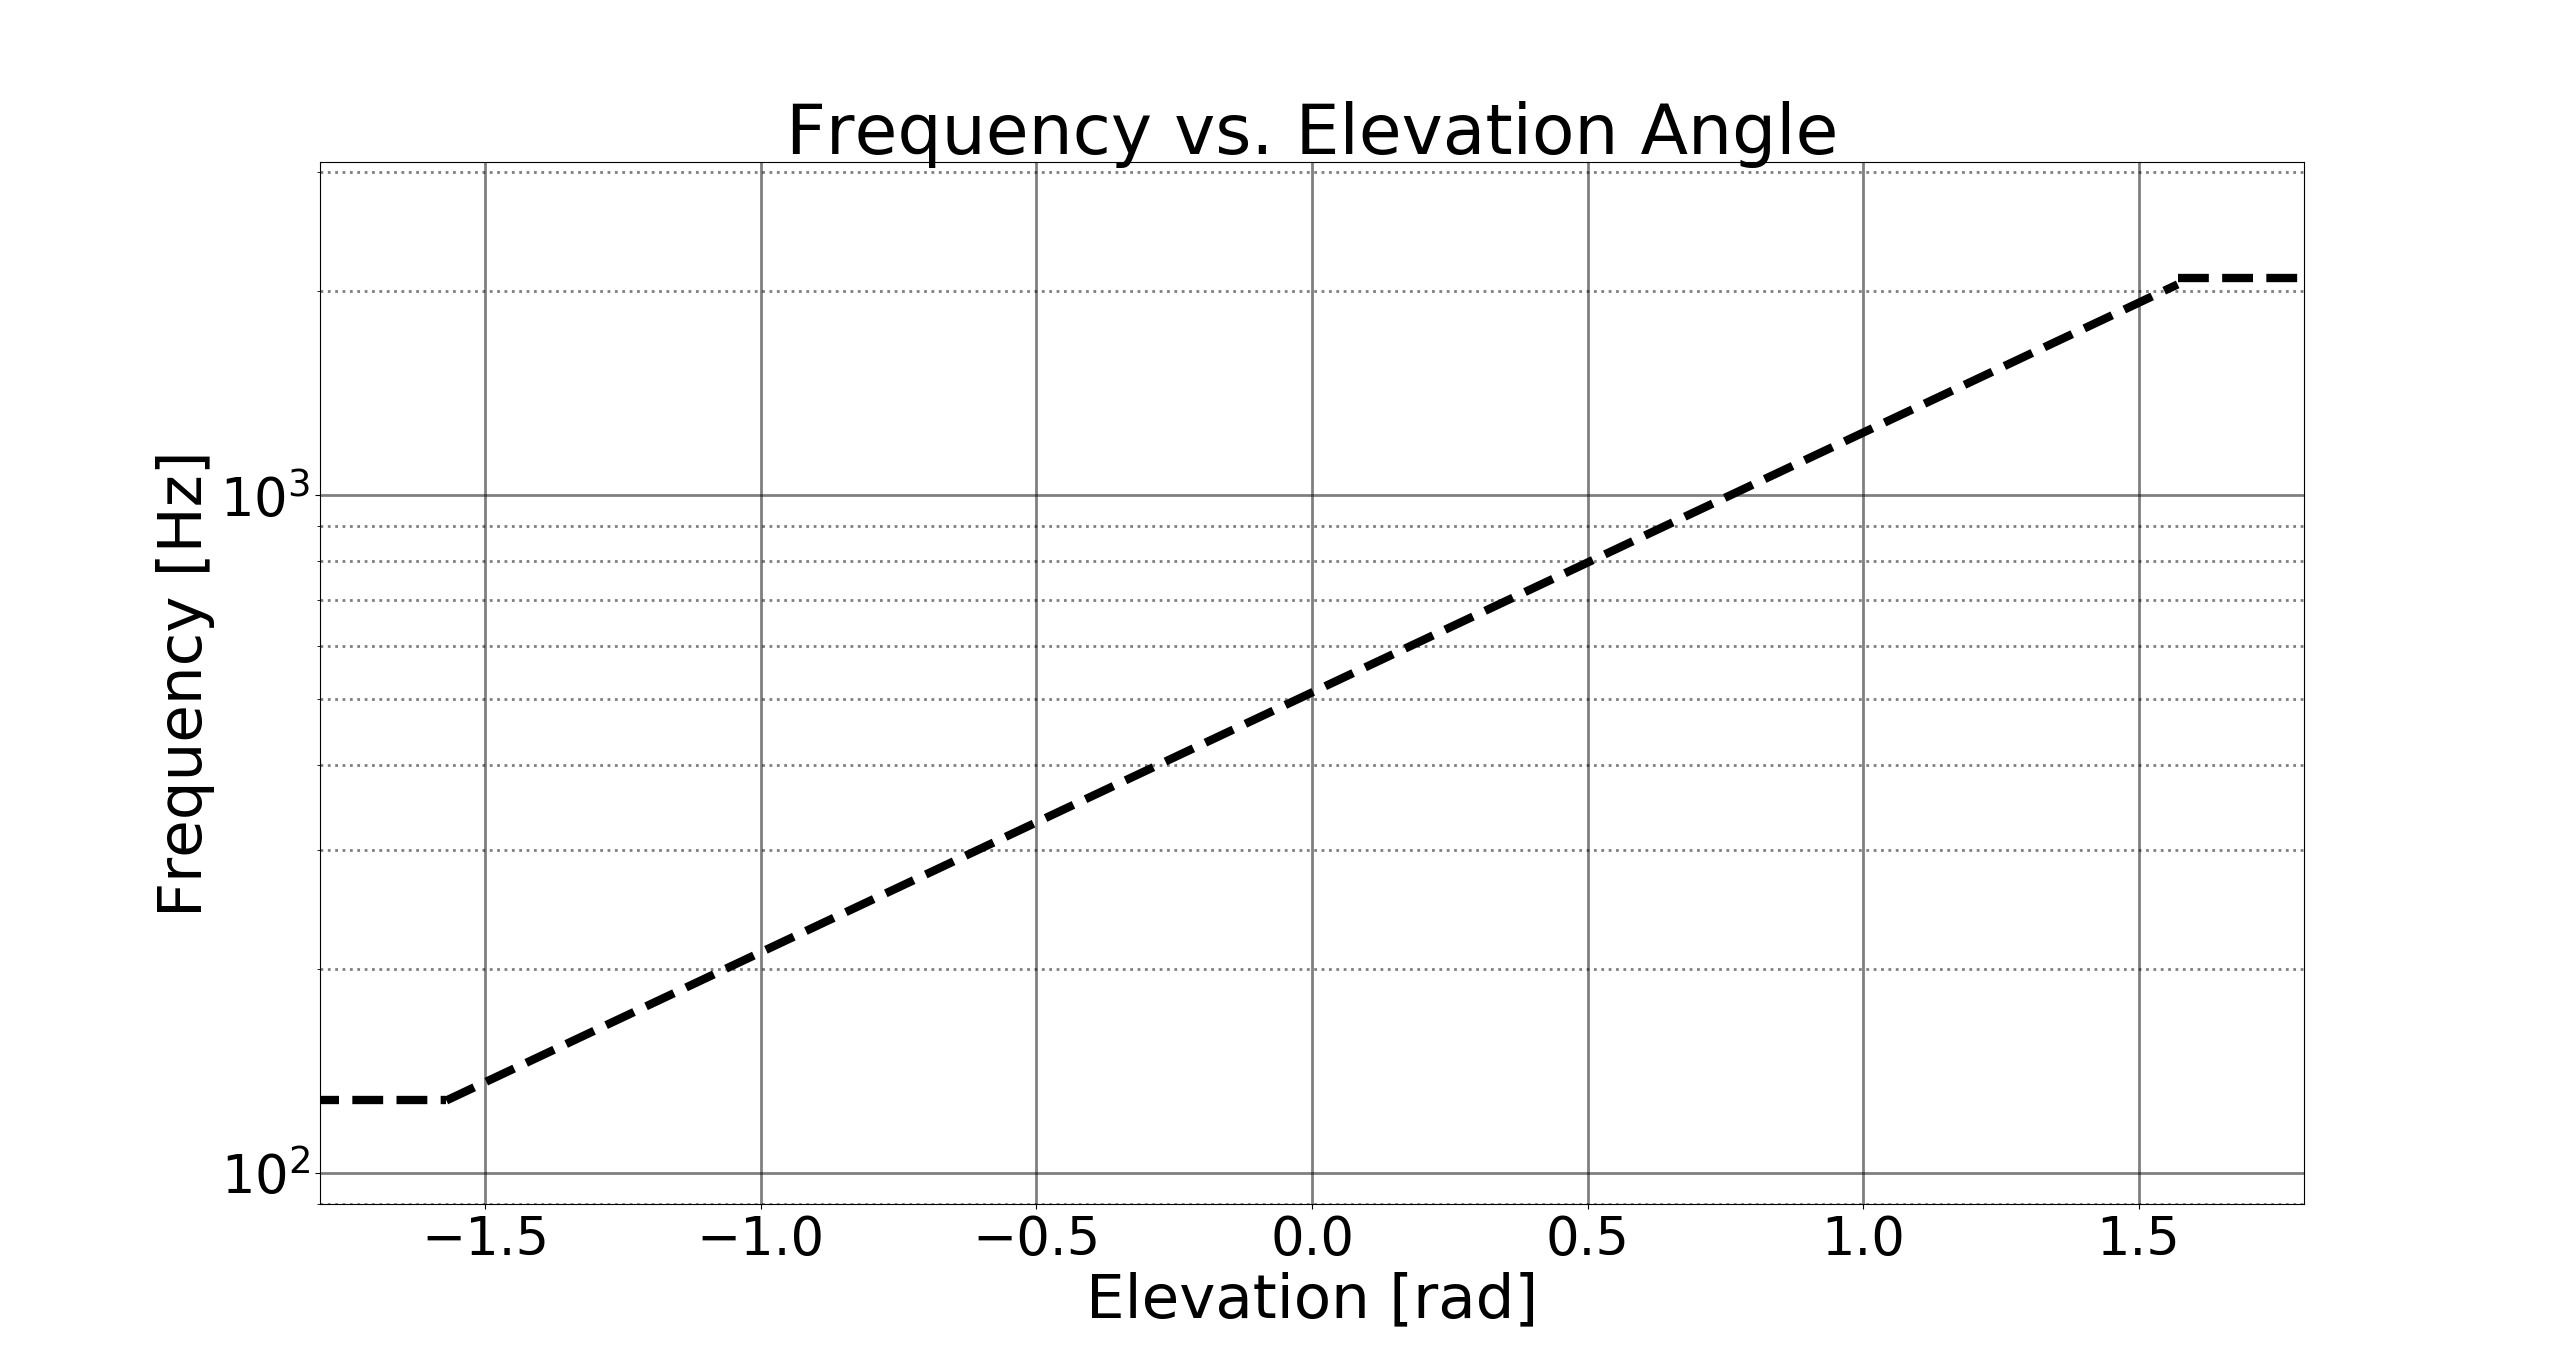
\includegraphics[clip, trim=0 0 0 40, width=0.6\columnwidth]{figures/pitch_gain_function.png}}
  \caption{The reference system used by the guidance interface showing the camera vector and pan and elevation angles (left) and the pitch gain function used to convey the target's elevation angle (right). Note the logarithmic scale of the frequency axis.}
\end{figure}

\subsubsection{Pan Dimension}

The human audition system uses binaural comparison cues, such as ITD and ILD, to localise a sound source on the horizontal plane~\cite{blauert1969sound}.
The ITD is the perceived time delay between the signal reaching both ears, while the ILD is the perceived volume difference in the signal.
For example, a sound that comes from the individual's right will hit the right ear first with a slightly higher volume.

In this work, a pure sinusoidal wave was used. 
People typically have trouble localising a pure tone without a sufficiently rich spectral signature.
However, the ITD and ILD are independent of the tone's spectral make-up, while the elevation angle is given through a different mechanism. Therefore, a pure sine wave is suitable to convey the target's pan angle.
To transform and spatialise the audio signal, we used OpenAL's default HRTF, based on the MIT's KEMAR dataset~\cite{hiebert2005openal}, which uses the person and targets' positions as input, and outputs a transformed audio signal.

\subsubsection{Elevation Dimension}

A generic HRTF implementation with bone-conduction headphones is not very effective in conveying the elevation angle of a sound source~\cite{macdonald2006spatial,schonstein2008comparison}.
To compensate for this, we communicate the target's elevation angle by adjusting the tone's pitch (i.e.\ the sine wave's frequency) as a function of the elevation. 
When the camera vector is at the correct elevation, the tone pitch is set to neutral.
When the target is above or below the camera vector, the pitch is increased or decreased, respectively.
This high/low association scheme is motivated by humans' natural association of high-pitched sounds with elevated sound sources, and low-pitched sounds with source's below the individual's earline~\cite{pratt1930spatial,blauert1997spatial}.
An octave- and semitone-based function is used to adjust the tone's pitch to ensure perceptible changes, while keeping the timbre roughly constant~\cite{shepard1964circularity}.
The pitch is updated at a rate of \SI{10}{\hertz} and changes as the user moves the device.

The pitch is changed as a linear function of the elevation angle and the gradient is determined by setting the angle and pitch limits.
For this work, we only consider a \SI{180}{\degree} field of view in front of the user and limit the elevation angle to a range of \SI{\pm90}{\degree}, or $[-\frac{\pi}{2}, \frac{\pi}{2}]$.
The pitch limits are set at some integer number of octaves above and below the neutral, on-elevation pitch.
After practical tests with the interface, we set the neutral pitch to \SI{512}{\hertz}, which is comfortably audible and allows for a large number of suitable octave limits to be selected.
We set the pitch limits to 2 octaves away from the neutral pitch, giving frequency limits of [\SI{128}{\hertz}, \SI{2048}{\hertz}].
The linear function is visualised in \cref{fig:pitch-gain}.

\section{Experiments}

\subsection{Implementation}

A diagram of the experimental system pipeline is shown in \cref{fig:pipeline}, where the arrows indicate the direction of the information flow.
When the user taps the Tango's screen, a new virtual target is generated and its coordinates are sent to the audio generation module, along with the device's current position and orientation.
The audio generator then produces a tone based on the difference between the device and the target's positions. The tone is sent to the audio output channel, which plays it back to the user.
A WiFi recording module is constantly monitoring the different values of the device's parameters and of the target's position, as well as the system's output, recording everything to a remotely stored datafile. 

\begin{figure}[t]
  \centering
  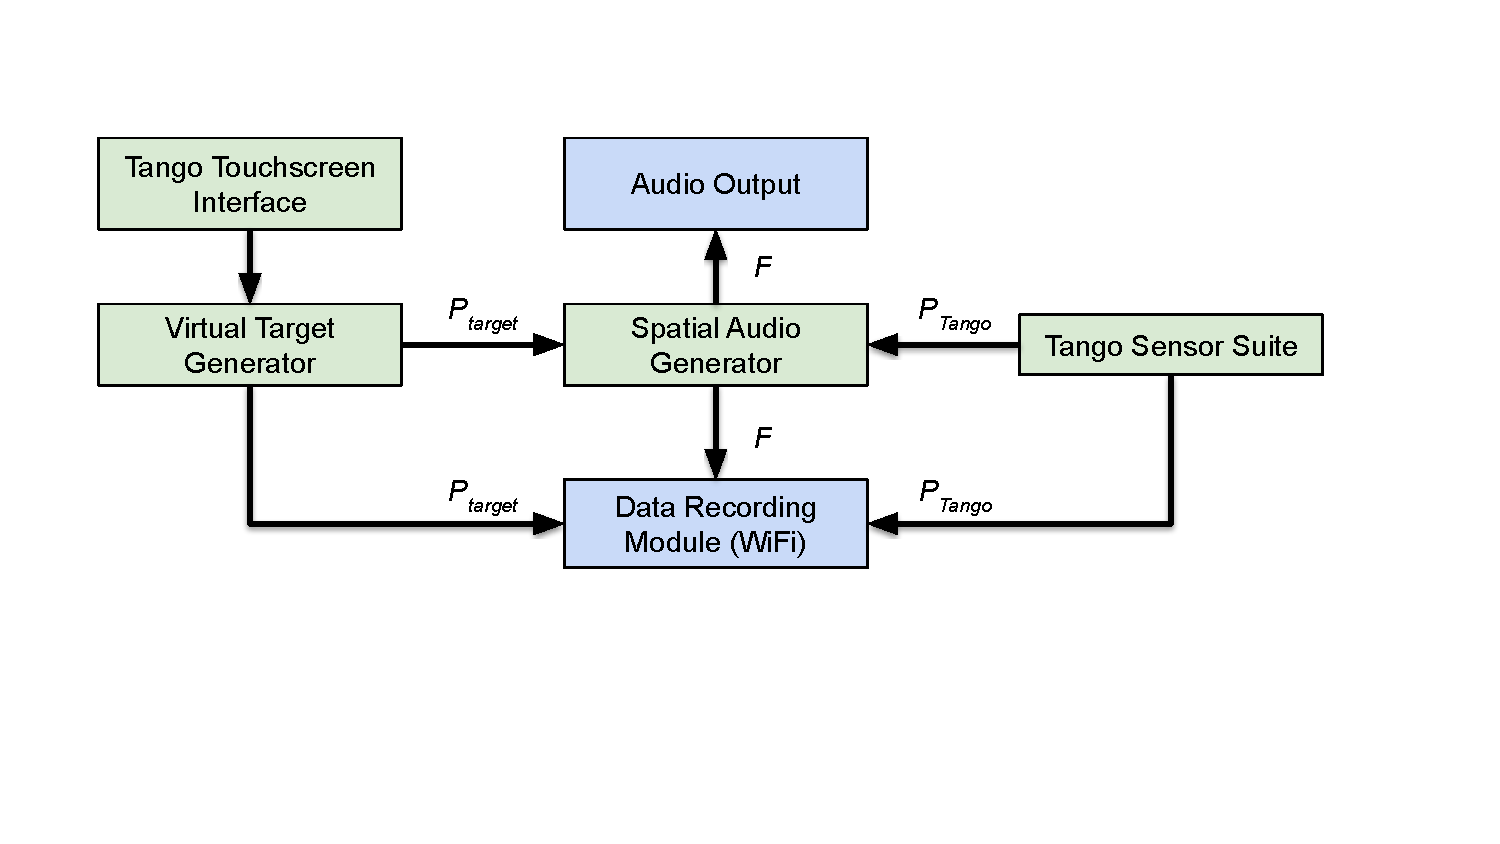
\includegraphics[clip=true, trim=0 120 80 50, width=0.9\columnwidth]{figures/pipeline.pdf}
  \caption{A diagram of the individual system components and their communication pipelines. $F$ indicates a feedback signal and $P$ a pose signal. }\label{fig:pipeline}
\end{figure}

\subsection{Participant Characterisation}

In addition to the target searching experiment, another set of experiments were conducted to characterise the participants' hearing characteristics.
The characteristics that were measured were each participant's audio localisation ability on the lateral plane, as well as the participants' ability to discriminate between tones with different frequencies. 
These results will be used to provide context to the results captured during the target search experiment and provide additional insight on any possible biases or limitations. 

\subsubsection{Sound Localisation}

In this experiment, we evaluated a participant's ability to determine the lateral direction a sound is coming from.
To do this, we played a continuous \SI{512}{\hertz} sinusoidal tone to the participant through the headphones and applied an HRTF to spatialise and place its source to the participant's left or right.
The participant then had to select the direction the sound came from.
The longer the experiment lasts and the more correct guesses the participant makes, the closer the source moves to the centre-front of the participant, making it progressively harder to localise. 

For this progressive increase in difficulty, a 2-up, 1-down step process is used~\cite{wetherill1965sequential,levitt1971transformed}, meaning that for every 2 correct answers, the distance to the centre halves.
Conversely, the task becomes easier for each incorrect answer by doubling the sound source's distance from the centre.
We also use 2 different step sequences, one starting at a large distance (\SI{45}{\degree}) from the user and the other at the minimum distance (approximately \SI{1}{\degree}), giving an `easy' and a `hard' progression respectively.
The terminating condition for the experiment is when the 2 sequences converge to within 2 intervals of one another for 3 consecutive guesses.
This gives a distance band within which the participant is capable of localising the sound source.
Each participant performed this experiment three times. 

\subsubsection{Pitch Discrimination}

Here we determined a participant's ability to differentiate the pitches of 2 tones being played to them, i.e.\ how well they can tell if a tone is high or low pitched.
We played 2 tones to the participants in succession with the second tone being higher or lower-pitched than the first.
The participants were then asked to select whether they interpreted the second tone as higher or lower-pitched than the first.

The first tone is randomly generated, while the second tone is generated by adding or subtracting some value from the first one.
The tone difference depends on how well the participant can tell the tones apart.
Like the sound localisation experiment, a 2-up, 1-down step process is used: for every 2 consecutive correct answers, the pitch difference between the tones is halved and is doubled for every incorrect answer.
2 step sequences are again used here, one starting with a large pitch difference ($f_h=2^9=$ \SI{512}{\hertz}) between the tones and the other with a small difference ($f_l=2^1=$ \SI{2}{\hertz}).
The termination condition is when the 2 step sequences are within 1 octave of each other (i.e.\ $\log_2\frac{f_h}{f_l}=2^1$) for 3 consecutive answers.
Each participant performed this experiment twice. 

\subsection{Target Search}

To test the interface's effectiveness at guiding the user in a pointing task, a set of experiments were conducted to capture the difference between the targets' actual direction and the directions the participants' perceived them to be.
The participants were given a Tango device running an app written for the experiment that generates a set of virtual targets and presents them to each participants, one at a time. 
The targets are generated at a constant distance from the participant and their pan and elevation angles are uniformly generated across the four quadrants of the pan-elevation plane to avoid clustering.
Each target's angular position is communicated to the participant through the audio interface, the output of which is adjusted in real-time as the participant points the device around. 
When a participant was confident that the device was on-target, i.e.~hearing the audio front-on at \SI{512}{\hertz}, they tapped the screen, marking the location and generating the next target.
The targets' positions are all set relative to the device's coordinate system, which is tracked using the Tango hardware and localisation API.\
A total of 28 targets were generated per participant. 

\subsection{Metrics}

We use two different metrics to compare the three different pitch gradient settings: the acquisition accuracy and search time.
The accuracy is given as the difference between the Tango's orientation at the time the participant confirmed they were on target, and the target's actual orientation.
We separate the results of the tilt and pan dimensions in order to see how the different pitch gradients affect a participant's pointing accuracy. 

We also compare the performance of the three pitch gradient settings in terms of the time it takes each participant to find a target.
However, since each participant was presented with a different, randomly generated set of targets, a direct time comparison is not possible.
Instead, we use Fitts's Law~\cite{fitts1954information}, modified by MacKenzie for uncertain target sizes and noisy data~\cite{mackenzie1992fitts}, which states that there is a relation between the time it takes to find a target and its index of difficulty (the ratio between the distance to the target and its width).
It also provides a so-called `index of performance' that we can use as a metric to compare the results between the three configurations. 

Here we briefly summarise the equations and quantities involved in our metric.
Fitts's Law is given by  

\begin{equation}
  \label{eq:fitts-base}
  t = a + bID,
\end{equation}

\noindent
where $t$ is the time it takes to find a target, $a$ and $b$ are constants determined through regression and $ID$ is a description of the difficulty of the target, given as logarithmic function of the ratio between the distance to the target and the target's width.
In our case, the targets have no width, since they are points in space, and we therefore use MacKenzie's modified form for $ID$, given by

\begin{equation}
  \label{eq:fitts-id}
  ID = \log_2\left(\frac{\theta}{w_e} + 1\right).
\end{equation}

\noindent
Here $\theta$ is the angular distance between subsequent target centres and $w_e$ is the targets' effective angular width~\cite{welford1968fundamentals}, given by

\begin{equation}
  \label{eq:fitts-we}
  w_e = \sqrt{2\pi e}\sigma = 4.133\sigma,
\end{equation}

\noindent
where $\sigma$ is the standard deviation of the error data, taken as the angle between the participant's target selection and target's actual angular position.
Fitts's index of performance, $IP$, can then be calculated using 

\begin{equation}
  \label{eq:fitts-performance}
  IP = \frac{ID}{t},
\end{equation}

\noindent
where $IP = \frac{1}{t}$ when $\sigma=0$.

\subsection{Procedure}

Two groups of participants were recruited for the experiments. 
Group \textit{G1} consisted of 42 young adults with normal eyesight who were blindfolded for the experiments, and group \textit{G2} contained 12 people with severe visual impairments. 
Both groups were given some time before the experiments to familiarise with the system, the audio signal's behaviour and the \SI{512}{\hertz} on-level tone. 
To minimise the speed/accuracy biases in the results, we asked the participants to focus on finding the targets, without worrying about the time it took. 

\section{Results}

\section{Conclusion}

\end{document}
